\section{Aufbau und Durchführung}
\subsection{Aufbau}
\label{sec:Aufbau}

\subsubsection{Versuchsaufbau für den ersten Versuchtsteil}
\label{sec:aufbau1}

Der Versuchsaufbau bestehe aus einem Mikrowellensteckplatz, welcher aus verschiedenen Bausteinen besteht.
Diese werden je nach Versuchsteil zusammengebaut.
Der als Erstes verwendete Aufbau ist in Abbildung \ref{fig:aufbau1} dargestellt.

\begin{figure}
  \centering
  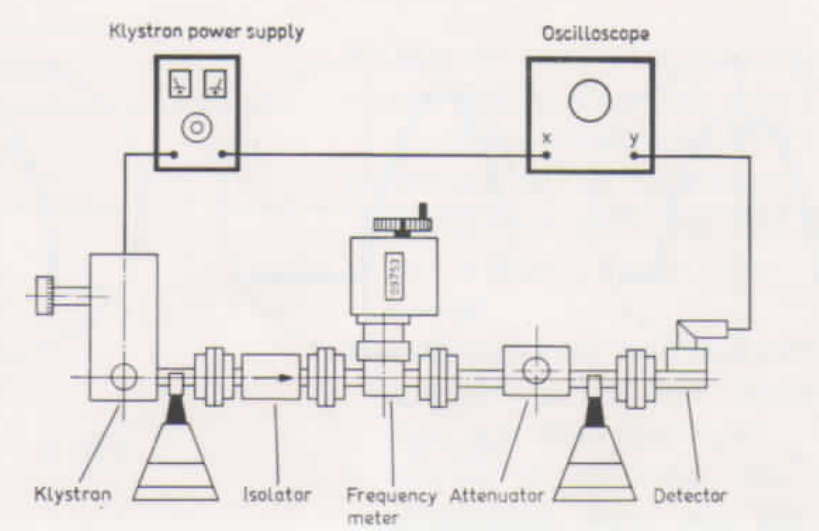
\includegraphics[height=7cm]{ressources/aufbau1.png}
  \caption{Skizze des Versuchsaufbaus für den ersten Aufgabenteil \cite{skript}.}
  \label{fig:aufbau1}
\end{figure}

Der Hauptteil des Versuches bildet ein rechteckiger Hohlleiter.
An dessen Anfang, in der Abbildung auf der linken Seite, befindet sich ein Reflexklystron zur Einspeisung der Mikrowellen.
Dessen genauer Aufbau wird in Kapitel \ref{sec:klysto} erläutert.
Das Klystron wird über eine Spannungsquelle versorgt, über die sowohl die Heizung für den Glühdraht als auch die Reflektorspannung geregelt werden.
Es folgt ein Isolator, dessen primärer Effekt es ist, eine Rückstrahlung von Mikrowellen in das Klystron zu vermeiden, was zu dessen Beschädigung führen würde.
Rechts davon wird ein Frequenzmesser angeschlossen, der auf eine feste Frequenz eingestellt werden kann.
Diese Einstellung führt bei übereinstimmender Frequenz von Mikrowellen und Frequenzmesser zu einer leichten Abschwächung des Signals.
Dieser Effekt in Verbindung mit einer Messaperatur wie dem Ozilloskop kann somit zur Messung der Mikrowellenfrequenz verwendet werden.
Als nächstes auf dem Hohlleiter befindet sich ein einstellbares Dämpfungsglied, welches das Signal abschwächt.
Über eine aufgedruckte logarithmische Skala kann die Schraubenstellung in die Dämpfungsstärke umgerechnet werden.
In diesem Versuchsteil wird der Hohlleiter durch einen Detektor abgeschlossen, welcher mit einer Diode ausgestattet ist.
Dessen Signal kann mithilfe eines Oslilloskopes ausgelesen werden.

\subsubsection{Versuchsaufbau für den zweiten Versuchtsteil}
\label{sec:aufbau2}

Der zum ersten Verusch leicht veränderte Versuchsaufbau ist in Abbildung \ref{fig:aufbau2} dargestellt.

\begin{figure}
  \centering
  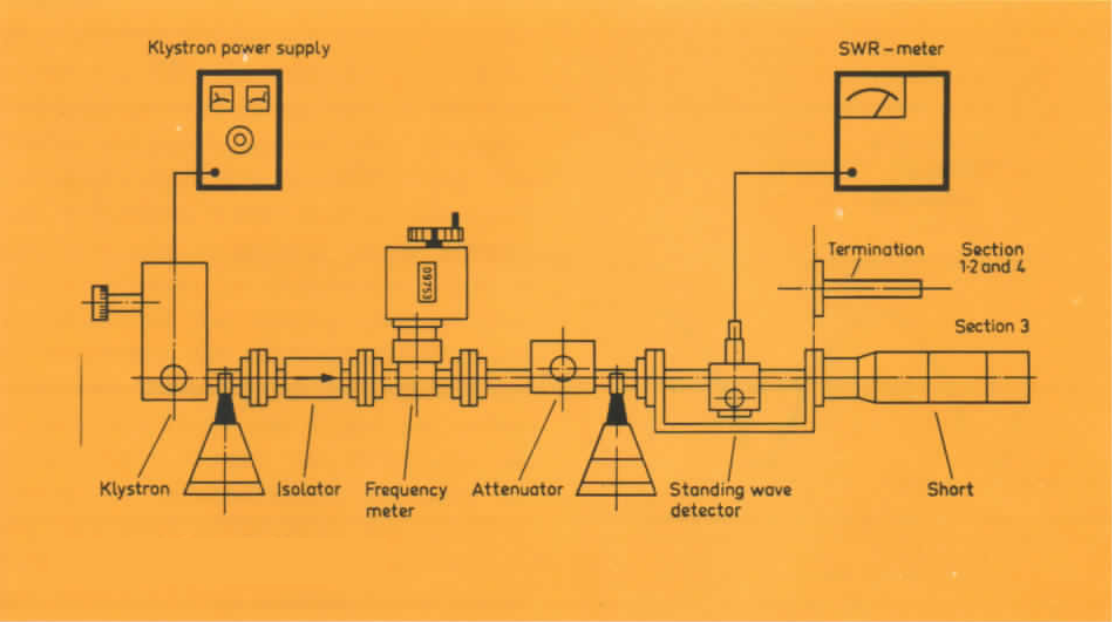
\includegraphics[height=7cm]{ressources/aufbau2.png}
  \caption{Skizze des Versuchsaufbaus für den zweiten Aufgabenteil \cite{skript}.}
  \label{fig:aufbau2}
\end{figure}

Während der Aufbau links vom Dämpfungsglied identisch bleibt, wird hinter ebendieses nun ein Stehwellen-Detektor geschaltet.
Dieser besteht aus einer Millimeterschiene, über die eine Sonde in den Hohlleiter eingeführt werden kann.
Die Tiefe der Sonde kann dabei variiert werden.
Das entnommene Signal wird an ein SWR-Meter weitergeleitet.
Mit diesem kann das Stehwellenverhältnis (siehe Kapitel \ref{sec:steh}) gemessen werden.
Das Ende Hohlleiters bildet entweder ein Kurzschuluss oder ein Abschluss, wodurch die Mikrowellen reflektiert bzw. absorbiert werden.

\subsubsection{Versuchsaufbau für den dritten Versuchtsteil}
\label{sec:aufbau3}

Für den dritten Versuchsteil wird wiederum ein leicht veränderter Aufbau vom zweiten Versuchsteil verwendet.
Dieser ist in Abbildung \ref{fig:aufbau3} skizziert.

\begin{figure}
  \centering
  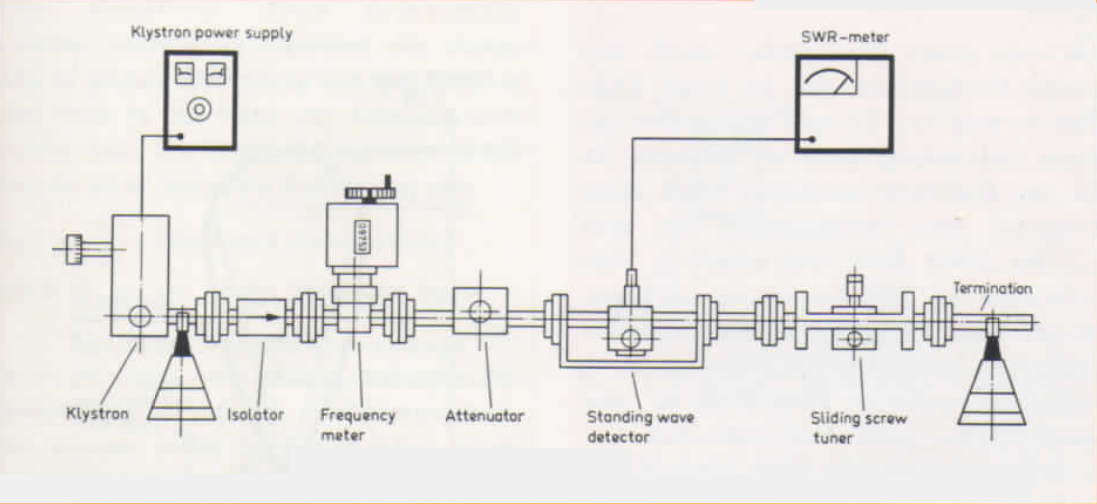
\includegraphics[height=7cm]{ressources/aufbau3.png}
  \caption{Skizze des Versuchsaufbaus für den dritten Aufgabenteil \cite{skript}.}
  \label{fig:aufbau3}
\end{figure}

Als Ende des Hohlleiters wird diesmal fest ein Abschluss gewählt.
Zwischen Abschluss und Stehwellendetektor wird jedoch noch ein Gleitschraubentransformator angebracht.
Dieser besteht aus einen Stift, welcher in den Hohlleiter mit variabler Tiefe eingeführt werden kann.
Über eine Schiene kann auch die horizontale Position eingestellt werden.
